%!TEX TS-program = xelatex
\documentclass[]{friggeri-cv}
\addbibresource{bibliography.bib}
\usepackage{fontawesome}  
\usepackage{graphicx}
\usepackage{enumitem}
\graphicspath{ {images/} }

\begin{document}
\header{miruna}{popa}
       {data scientist}

% In the aside, each new line forces a line break
\begin{aside}
  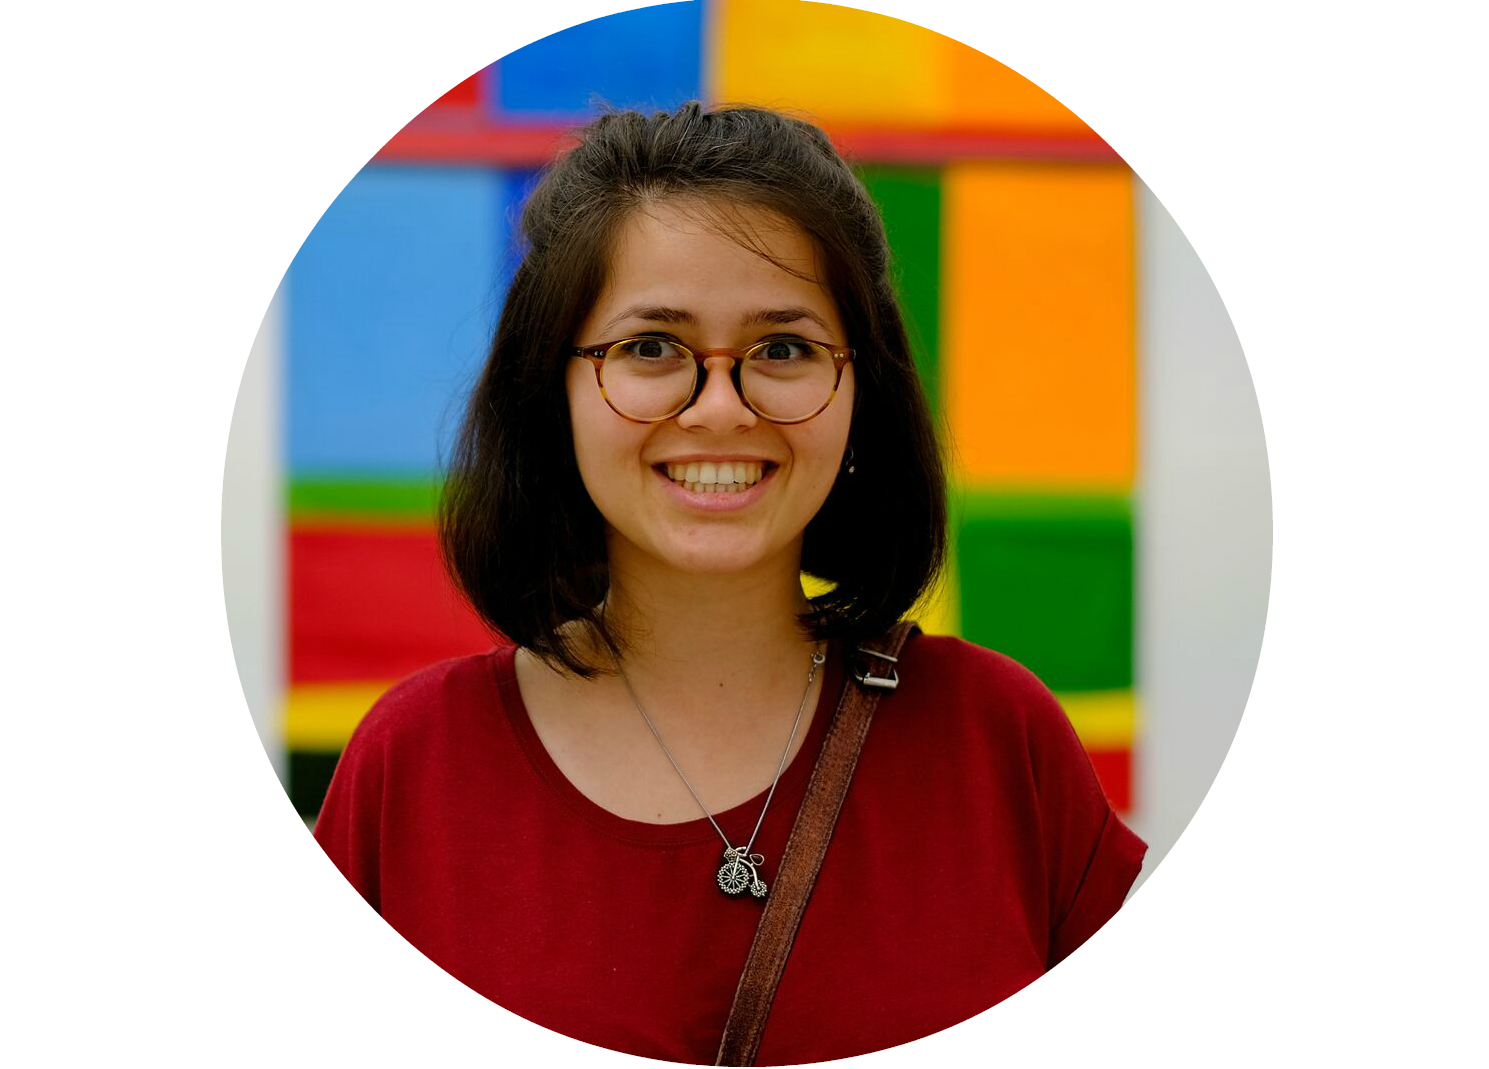
\includegraphics[width = 3cm, height = 3cm, keepaspectratio=true]{reedited_photo.png}
  ~
  \section{about}
  ~
    Zehdenicker Str. 15
    10119 Berlin
    Deutschland
    ~
    {\color{lightgray} \faEnvelope \href{mailto:miruna.c.popa@gmail.com} {  miruna.c.popa\\@gmail.com}}
    {\color{lightgray} \faMobilePhone {  +4917656977157}}
    ~
    {\color{lightgray} \faGithub \href{https://www.github.com/mirunapopa} {  mirunapopa}}
    {\color{lightgray} \faLinkedin \href{https://www.linkedin.com/in/mirunapopa}{   mirunapopa}}
    ~

  \section{data}
    {\color{red}  \faHeart { Python, Spark Scala, PostgreSQL, Redshift}}
    {\textbf{Data Engineering} {Hands on experience with EMR, Hadoop, S3, HDFS}}
    {\textbf{Data Communications} {Chartio, Metabase, Jupyter Notebooks, Google Spreadsheets}}
    {\textbf{Python}\\ {Pandas, Numpy, Scikit-learn \& SciPy}}
    {\textbf{Stats} \\{Experience with AB test design: significance testing, power calculations, bootstrapping}}
    {Fiddled with: SAS, Systat, HTML, CSS, Latex}
  ~

  \section{languages}
    romanian (native)
    english (fluent)
    german (beginner)
    spanish \& french notions
\end{aside}

\section{summary}

Experience in data management within fast-paced startup environments and eager to nourish a data driven mentality. Seeking challenging environments with creative and curious people, a place from which one never stops learning. 

\section{experience}

\begin{entrylist}
  \entry
    {2014 - Present}
    { EyeEm GmbH, Berlin}
    {Data Scientist}
    {\begin{itemize}
    \item experience in translating business requirements in technical requirements
    \item preparing ETLs: from designing them, implementation, scheduling \& documentation (technical \& non-technical)
    \item helping on improving our search engine with:
      {\begin{itemize}
        \item performance dashboards (through a star schema designed for this purpose)
        \item evaluations
        \item constant communication with our R\&D Department for further research work which could be applied
        \item communication with the Platform team for implementing results of the evaluations into production
      \end{itemize}}
    \item set up the first data crunching repository in the company - reducing 5 cumulated work days to 1
    \item created an internal automated emailing system - sending out raw data to the Photography team on a desired basis - unblocked waiting time for the Photography team
    \item initiated a monthly internal newsletter - led multiple teams to do the same
    \item reduced time on uploading Spark Jars to EMR from 20 minutes to 2 minutes - 10x improvement on waiting time for the team
    \item created a slack bot which would answer some frequently asked questions - won the Internal Hackathon out of 15 teams
    \item pushing for internal study groups, finishing {\color{lightgrey}\href{https://www.springboard.com/workshops/data-science-intensive} {Data Science Intensive Course}}
    \item handling internal requests and improving the process
    \item onboarded the current data team (currently made of 6 people)
    \end{itemize}}

  \entry
    {07-10 2013}
    {Softgames GmbH, Berlin}
    {Internship QA}
    {\begin{itemize}
    \item testing games and improving QA process
    \item developing data-driven ad campaigns
    \item new user funnel analysis
    \item working closely with product managers and external partners on the development of games
    \end{itemize}}

\end{entrylist}

\pagebreak

\section{education}

\begin{entrylist}
  \entry
  {2011-2014}
  {B.S. in Economic Cybernetics,\\ 
  Statistics and Informatics} % Degree
  {Academy of Economic Studies, Bucharest, Romania} % Institution
  {\emph{Final  Thesis:  Music  Recommendation  Web  App using  Collaborative Filtering Algorithm and Scala Programming Language}}

  \entry
  {2013–2014}
  {Erasmus Student in\\
  Computer Science\\
  and Economics}
  {West Pomeranian University of Technology,  Szczecin, Poland}
  {Topics Studied: Data Analysis \&  Machine Learning, Java Programming, Economic Analysis}
  
\end{entrylist}

\section{volunteering}

\begin{itemize}
  \item
  {2011-2013}
  {\textbf{Volunteers for Ideas and Projects, Bucharest}: dealt with Marketing, Sales, Art Direction}
  \item
  {2007-2010}
  {\textbf{Ingenious Drama Festival, Bacau}: Chief of Magazine Department & awarded Most active member of the Department
\end{itemize}

\end{document}